% Chapter Template

\chapter{Introduction} % Main chapter title

\label{Chapter1} % Change X to a consecutive number; for referencing this chapter elsewhere, use \ref{ChapterX}

\lhead{Chapter 1. \emph{Introduction}} % Change X to a consecutive number; this is for the header on each page - perhaps a shortened title

%----------------------------------------------------------------------------------------
%	SECTION 1
%----------------------------------------------------------------------------------------

%############################# Introduction #################################
\section{Background}
  Concrete is the synthetic material currently produced in volumes larger than any other material on Earth. With an annual consumption of approximately 35 billion tonnes, it is only second to water in terms of global usage\supercite{Monteiro2017, VanDamme2018}. As the backbone of modern infrastructure, it provides the foundations for buildings, bridges, roads, dams, and other structures essential for societal development. Its widespread adoption arises from a unique combination of strength, versatility, and cost-effectiveness\supercite{Mehta2014}, rendering it indispensable to the construction industry.

  Nevertheless, despite the ubiquity of concrete, the properties of its key constituent, cement, remain incompletely understood. Cement is a chemically complex material, composed of a heterogeneous mixture of minerals that undergo a series of hydration reactions upon contact with water. The principal product of cement hydration---and the primary binding phase of concrete--- calcium silicate hydrate (C-S-H) is the responsible for the mechanical strength, chemical and transport properties and durability of hardened cement paste and, consequently, of concrete itself\supercite{Papatzani2015, Ioannidou2016, Qomi2020, Bahraq2022}. Therefore, understanding the atomic and mechanical properties of C-S-H is of the uttermost importance to better formulate cementitious materials with enhanced performance and durability. Introduce here



%-----------------------------------
%	SUBSECTION 1
%-----------------------------------
\section{Problem Statement}

Nunc posuere quam at lectus tristique eu ultrices augue venenatis. Vestibulum ante ipsum primis in faucibus orci luctus et ultrices posuere cubilia Curae; Aliquam erat volutpat. Vivamus sodales tortor eget quam adipiscing in vulputate ante ullamcorper. Sed eros ante, lacinia et sollicitudin et, aliquam sit amet augue. In hac habitasse platea dictumst.

%-----------------------------------
%	SUBSECTION 2
%-----------------------------------

\section{General and Specific Objectives}
Morbi rutrum odio eget arcu adipiscing sodales. Aenean et purus a est pulvinar pellentesque. Cras in elit neque, quis varius elit. Phasellus fringilla, nibh eu tempus venenatis, dolor elit posuere quam, quis adipiscing urna leo nec orci. Sed nec nulla auctor odio aliquet consequat. Ut nec nulla in ante ullamcorper aliquam at sed dolor. Phasellus fermentum magna in augue gravida cursus. Cras sed pretium lorem. Pellentesque eget ornare odio. Proin accumsan, massa viverra cursus pharetra, ipsum nisi lobortis velit, a malesuada dolor lorem eu neque.

%----------------------------------------------------------------------------------------
%	SECTION 2
%----------------------------------------------------------------------------------------

\section{Overview}

Sed ullamcorper quam eu nisl interdum at interdum enim egestas. Aliquam placerat justo sed lectus lobortis ut porta nisl porttitor. Vestibulum mi dolor, lacinia molestie gravida at, tempus vitae ligula. Donec eget quam sapien, in viverra eros. Donec pellentesque justo a massa fringilla non vestibulum metus vestibulum. Vestibulum in orci quis felis tempor lacinia. Vivamus ornare ultrices facilisis. Ut hendrerit volutpat vulputate. Morbi condimentum venenatis augue, id porta ipsum vulputate in. Curabitur luctus tempus justo. Vestibulum risus lectus, adipiscing nec condimentum quis, condimentum nec nisl. Aliquam dictum sagittis velit sed iaculis. Morbi tristique augue sit amet nulla pulvinar id facilisis ligula mollis. Nam elit libero, tincidunt ut aliquam at, molestie in quam. Aenean rhoncus vehicula hendrerit.

\begin{figure}[H]
    \centering
    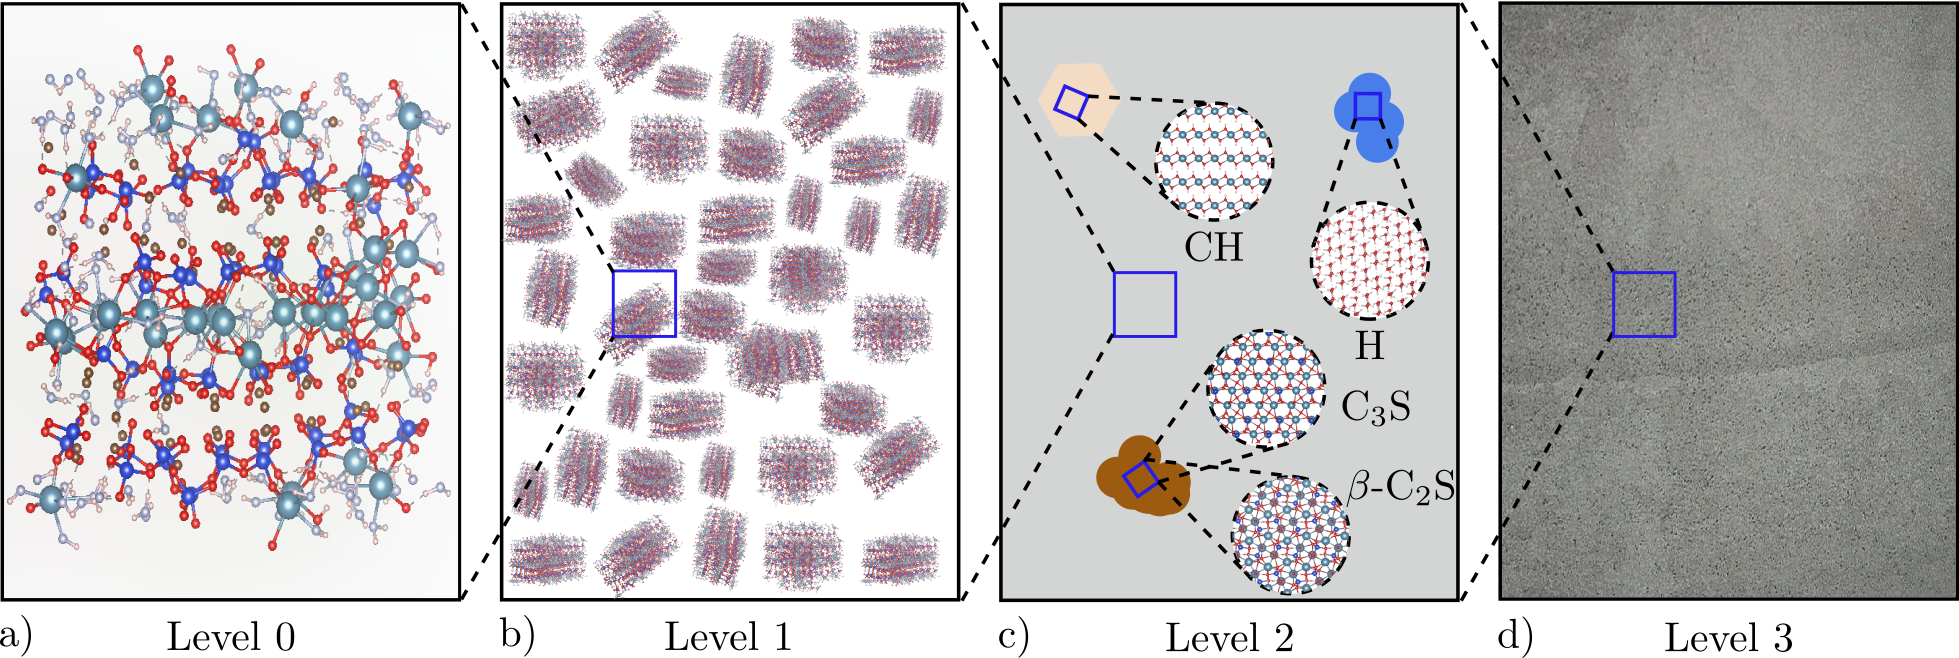
\includegraphics[width=0.8\textwidth]{levels.png}
    \caption{Caption of the figure.}
    \label{fig:figure1}
\end{figure}


